\chapter{Inelastic Cosmic Ray Collisions}\label{chap:cr}

Dark Matter direct detection experiments lose sensitivity to sub-GeV particles due to prohibitively small nuclear recoil energies. On the other hand, previous work such as ~\cite{Bringmann:2018cvk, Ema:2018bih} suggests that light dark matter may naturally lead to a sub-dominant flux of higher momenta particles. This would lead to a reinterpretation of the current direct detection limits. Here we present a calculation of such a flux arising from inelastic cosmic ray collisions in the atmosphere. We also derive limits from the XENON1T experiment and forecast the reach of the LZ detector.

\section{Cosmic Ray Dark Matter Flux}
We distinguish two possible sources for a dark matter flux arising from the mechanism described in the Introduction: inelastic cosmic ray collisions with protons in the interstellar medium and with the atmosphere on Earth. According to our calculations, the former yields a flux several orders of magnitude lower than the latter; therefore, we may safely neglect it and focus on our modelling of interactions at the atmosphere. 

The incoming cosmic ray flux is taken to be the local interstellar proton spectrum parametrised as in Ref.~\cite{Boschini:2017fxq}; alternatively we have also checked that using the AMS02 spectrum~\cite{Consolandi:2014uia} leads to identical results. The differential intensity $dI/dR$ as a function of particle rigidity $R$ is converted to a flux $d\Phi_p / dT_p = 2\pi (dR/dT_p)(dI/dR)$ per unit area, time, and kinetic energy $T_p$, over a hemispherical solid angle. We performed a Monte-Carlo simulation of this incoming flux using EPOS-LHC~\cite{Pierog:2013ria}, as implemented in the CRMC package~\cite{CRMC}, to simulate the collisions assuming the atmospheric nuclei target to be nitrogen at rest. The resulting $\pi^0$ and $\eta$ mesons undergo two subsequent two-body decays via a vector or scalar mediator~\footnote{Here we consider only on-shell mediators though the sensitivity could in principle be extended to heavier off-shell mediators.} to a pair of dark matter particles, with a branching ratio that we keep as a free parameter. The rate of interactions is then integrated as follows over the volume of the atmosphere to obtain the total dark matter flux at the detector. 

\begin{figure}[t]
\begin{center}
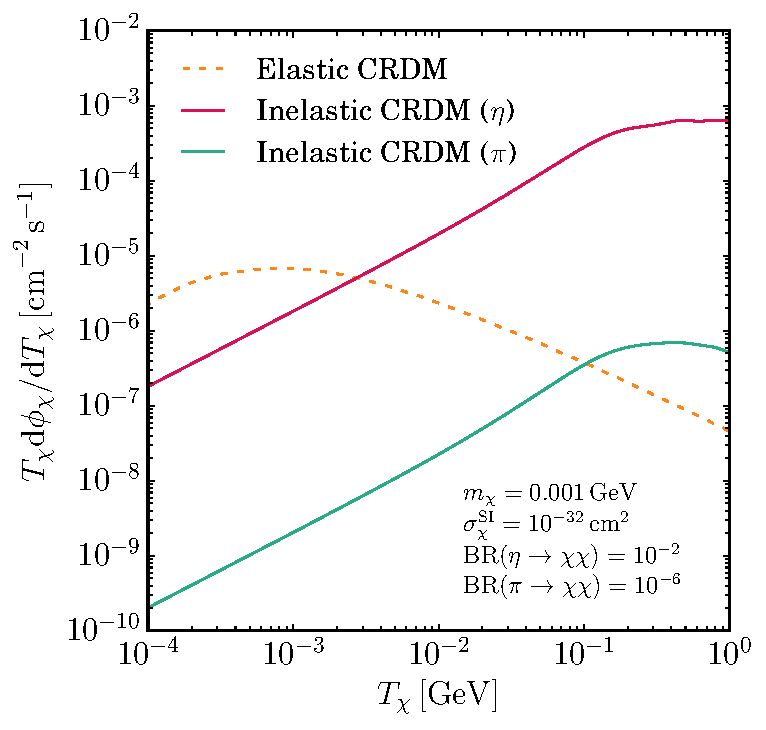
\includegraphics[width=0.6\textwidth]{pion_eta_chi_no_title.pdf}
\end{center}
\caption{Dark matter flux from cosmic rays for elastic collisions in dotted orange with $m_\chi = 1$ MeV, and for inelastic collisions with $BR(\pi^0 \to \chi \chi + ...) = 10^{-6}$ in solid green and $BR(\eta \to \chi\chi + ...) = 10^{-2}$ in solid red.
\label{fig:flux}}
\end{figure}

The differential cosmic ray flux gets attenuated through the atmosphere as a function of height $h$ from ground level: 
%
\begin{equation}
\frac{d}{dh}\left(\frac{d\Phi_p}{dT_p}\right) = \sigma_{pN}(T_p) n_N(h) \frac{d\Phi_p}{dT_p} \, ,
\label{eq:diff}
\end{equation}
%
where $\sigma_{pN}$ is the inelastic proton-nitrogen cross-section and $n_N$ is the number density of air, taken from Ref.~\cite{Jursa:1985}, which is assumed to be entirely nitrogen for simplicity. \eqref{eq:diff} neglects higher order effects such as regenerations and secondary scatterings involved in a detailed cosmic ray shower model, but it is sufficient to provide a conservative estimate of our hidden sector flux. Since $\sigma_{pN} \simeq 255$ mb is constant to a good approximation over the relevant energy range, we may write $\frac{d\Phi_p}{dT_p}(T_p,h) \equiv y(h) \cdot \frac{d\Phi_p}{dT_p}(T_p)$ and solve for the attenuation factor $y(h)$. The dark matter flux at a detector located at a depth $z_d$ below ground is then given by
%
\begin{align} \frac{d \Phi_{\chi}}{d T_{\chi}} &=\int_{R_{E}}^{R_{E}+h} R^{2} d R \int_{0}^{2 \pi} d \phi \int_{\cos \theta_{\max }}^{1} \frac{d(\cos \theta)}{2 \pi l\left(R, \theta, z_{d}\right)^{2}} \nonumber \\ & y\left(R-R_{E}\right) \frac{d \Phi_{p}}{d T_{p}} n_{N}\left(R-R_{E}\right) \sigma_{p N \rightarrow M} B R_{M \rightarrow \chi \chi} \equiv \frac{d \Phi_{p}}{d T_{p}} n_{N}^{0} H_{\mathrm{eff}} \sigma_{p N \rightarrow M} B R_{M \rightarrow \chi \chi} \label{eq:integratedflux}\end{align}
where $R_E$ is the radius of the Earth and $\theta_{\mathrm{max}}$ is a maximum angle dependent on the path length attenuation through the Earth, as described in the next Section. The line of sight distance $l(R,\theta, z_d)$ is given by 
%
\begin{equation}
l^2 = (R_E - z_d)^2 + R^2 - 2(R_E - z_d)R \cos{\theta} \, .
\end{equation}
%
It determines the rate dilution factor in the emission from source to detector that we have conservatively assumed to be isotropically distributed over a hemisphere. In the last line of \eqref{eq:integratedflux} we defined an equivalent effective height at a constant number density taken to be the ground-level value, $n_N^0 \simeq 5\times 10^{19} \mathrm{ cm}^{-3}$~\cite{Jursa:1985}. For example, with $\cos\theta_{\mathrm{max}} = -1$, i.e. the Earth completely transparent to dark matter, we obtain $H_{\mathrm{eff}} \simeq 5$ km. 

The resulting dark matter flux in the transparent Earth case is plotted in Fig. \ref{fig:flux} in solid red for $BR(\eta \to \chi \chi + ...) = 10^{-2}$ and green for $BR(\pi^0 \to \chi\chi + ...) = 10^{-6}$, close to their experimental upper limits. The fluxes are rather insensitive to the mediator and dark matter masses when these are produced on-shell. For comparison, we show in dotted orange the up-scattered flux for $m_\chi = 1$ MeV coming from elastic collisions of cosmic rays with interstellar dark matter, calculated as in Ref.~\cite{Bringmann:2018cvk}. Finally we have also checked that, when restricting to an opaque Earth, the muon flux obtained in our approach is in good agreement with data~\cite{Haino:2004nq,Tanabashi:2018oca}.

\section{Attenuation through the Earth}

As dark matter travels from the point of production through the Earth a large enough nucleus interaction cross-section can prevent it from reaching the detector. The mean free path length together with the line of sight distance through the Earth to the detector then determines the maximum polar angle at which we cut off the atmospheric volume integral in \eqref{eq:integratedflux}. This line of sight distance through the Earth is given by
%
\begin{align}
l_E &= \frac{1}{2}\left( b + \sqrt{b^2 + 4(R_E^2 - (R_E - z_d)^2)} \right) \, , \nonumber \\
b &\equiv \text{Sign}\left[R_E - z_d - (R_E + h)\cos\theta \right]  \nonumber \\
& \quad \quad \quad \times 2(R_E - z_d) \sqrt{1 - \frac{(R_E +h)^2 \sin^2\theta}{l^2}} \, .
\end{align}
%

The mean free path length is determined by solving for the kinetic energy loss assuming a uniform distribution of nuclear recoil energy in elastic scattering, $d\sigma_{\chi N}/dT_r = \sigma_{\chi N} / T_r^{\mathrm{max}}$, following Ref.~\cite{Bringmann:2018cvk}. Summing over the nuclei $N$, we then have
%
\begin{align}
\frac{dT_\chi}{dz} &= - \sum_N n_N \int_0^{T_r^{\mathrm{max}}} \frac{d\sigma_{\chi N}}{dT_r} T_r dT_r \nonumber \underset{(T_\chi \ll m_N) }{\simeq} -\frac{1}{2m_\chi L}\left(T_\chi^2 + 2 m_\chi T_\chi \right) \, ,
\end{align}
%
where we used
%
\begin{equation}
T_r^{\mathrm{max}} = \frac{T_\chi^2 + 2m_\chi T_\chi}{T_\chi + (m_\chi + m_N)^2/(2m_N)} \, ,
\end{equation}
%
and defined the mean free path length
%
\begin{equation}
L \equiv \left( \sum_N n_N \sigma_{\chi N} \frac{2 m_N m_\chi}{(m_\chi + m_N)^2} \right)^{-1} \, .
\end{equation}
%
Integrating this equation gives the incoming energy $T_\chi^0$ that is required to arrive at the detector with energy $T_\chi^z$ a distance $l_E$ through the Earth:
%
\begin{equation}
T_\chi^0 = \frac{2 m_\chi T_\chi^z e^{l_E/L}}{2 m_\chi + T_\chi^z(1-e^{l_E/L})} \, .
\end{equation}
%
From this we obtain $\theta_{\mathrm{max}}$ when $T_\chi^0 \to \infty$. The mean free path length is calculated by summing over the average number density of the elements given in Table 2 of Ref.~\cite{Kavanagh:2016pyr}. We relate the nuclear interaction cross-section to the per nucleon spin-independent cross-section $\sigma_\chi^{\mathrm{SI}}$ as
%
\begin{equation}
\sigma_{\chi N} = \sigma_\chi^{\mathrm{SI}} A^2 \left(\frac{m_N}{m_p} \frac{(m_\chi + m_p)}{(m_\chi + m_N)} \right)^2 \, .
\end{equation} 
%

In practise we find that at the depth of the XENON1T detector the attenuation starts cutting off the atmospheric volume integral for cross-sections above $\sigma_\chi^{\mathrm{SI}} \gtrsim 10^{-32} \, \mathrm{cm}^2$, with transmission falling exponentially above $\sim 10^{-28} \, \mathrm{cm}^2$.

\section{Limits}

Finally, we obtain the expected rate at a detector coming from our inelastic cosmic ray dark matter flux by integrating within the detector nuclear recoil thresholds $T_1$ and $T_2$:
%
\begin{equation}
\Gamma_N = N_T \int_{T_1}^{T_2} dT_N \int_{T_\chi^{\mathrm{min}}(T_N)}^\infty dT_\chi \epsilon(T_N) \frac{d\Phi_\chi}{dT_\chi} \frac{d\sigma_{\chi N}}{dT_N} \, ,
\end{equation}
%
where $N_T$ is the number of target atoms, $\epsilon$ is the detector nuclear recoil energy efficiency, and
%
\begin{equation}
T_\chi^{\mathrm{min}} = \left(\frac{T_N}{2} - m_\chi \right)\left(1 \pm \sqrt{1 + \frac{2T_N}{m_N}\frac{(m_\chi + m_N)^2}{(2m_\chi - T_N)^2}} \right) \, ,
\end{equation}
%
with a plus sign if $T_\chi > 2m_N$ and minus sign otherwise. As an illustrative example we will focus on the limits from XENON1T. Its nuclear recoil energy threshold window is from $T_1 = 4.9$ keV to $T_2 = 40.9$ keV and the detector is located at a water-equivalent depth of 3.6 km, corresponding to 1.4 km of rock~\cite{Aprile:2018dbl}. For the 90\% CL limits we require a total number of events $N_{90\% \text{ CL}} = 3.56$ for the full exposure of 278.8 days of data collection with 1.3t fiducial mass. This event count, in Table 1 of Ref.~\cite{Aprile:2018dbl}, is the best fit given by a likelihood analysis for a 200 GeV WIMP whose recoil spectrum is comparable to that of the energetic light dark matter flux. 

\begin{figure}
\begin{center}
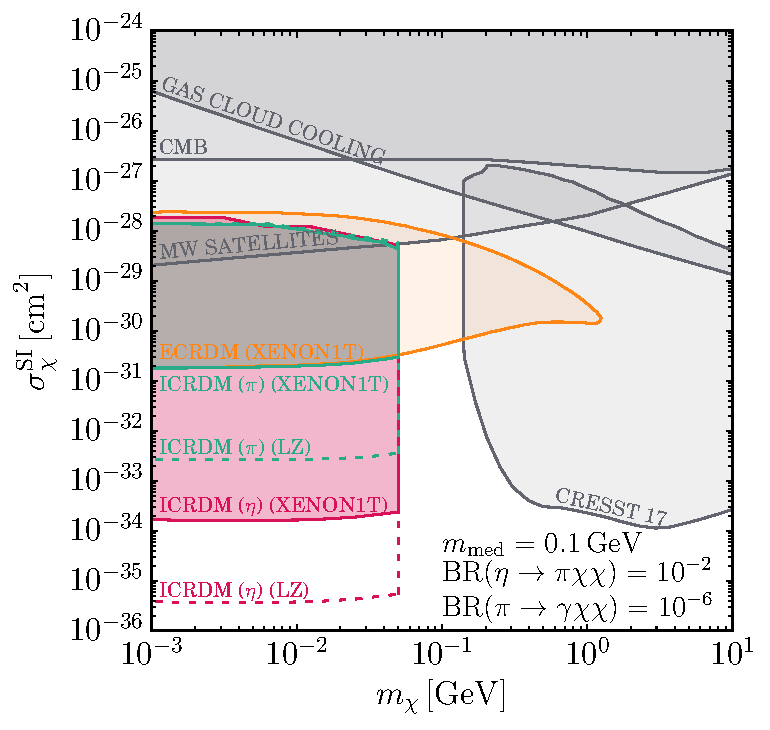
\includegraphics[width=0.615 \textwidth]{sigma_mchi_eta_pi_no_title.pdf} \\
\hspace{-0.25cm}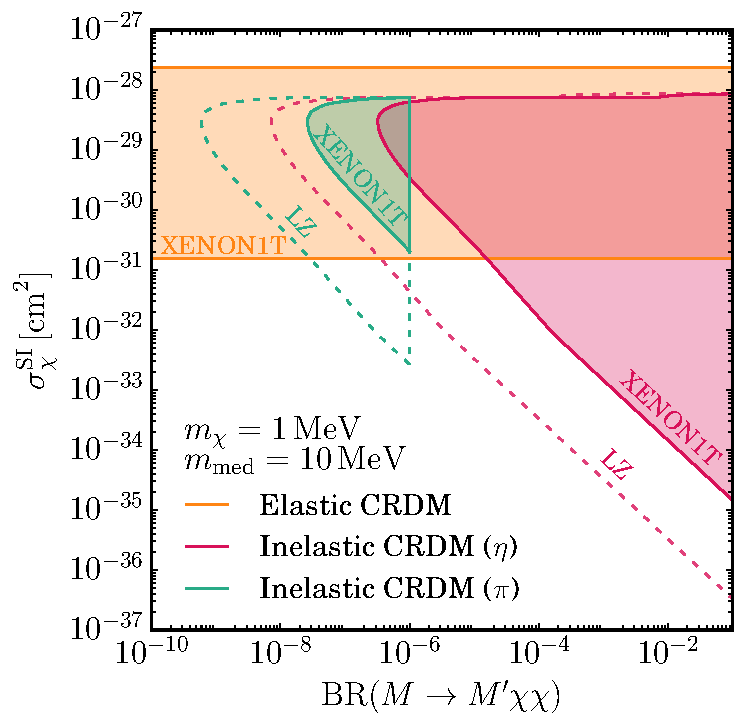
\includegraphics[width=0.6 \textwidth]{limit_no_title.pdf}
\end{center}
\caption{90\% CL limits on the spin-independent dark matter-nucleon cross-section as a function of dark matter mass for a fixed branching ratio (\textit{top}) and as a function of branching ratio for a fixed dark matter mass (\textit{bottom}), as labelled. The inelastic cosmic ray dark matter limits from XENON1T~\cite{Aprile:2018dbl} are indicated in red and green for the flux originating from meson $M=\eta$ and $\pi^0$ decays, respectively, and in orange for elastic cosmic ray dark matter. The dashed lines are projections for the future LZ experiment~\cite{Akerib:2018lyp}. Other limits in grey are taken from Ref.~\cite{Bringmann:2018cvk} (based on CRESST~\cite{Angloher:2017sxg}, CMB~\cite{Xu:2018efh}, and gas cloud cooling~\cite{Bhoonah:2018wmw}), and from Milky-way satellites~\cite{Nadler:2019zrb}. 
\label{fig:limits}}
\end{figure}


For comparison with Ref.~\cite{Bringmann:2018cvk}, we first assume a uniform recoil energy distribution, $d\sigma_{\chi N}/dT_N = \sigma_{\chi N} / T_{r,N}^{\mathrm{max}}$, and similarly obtain the resulting XENON1T limits on $\sigma_\chi^{\mathrm{SI}}$. This is plotted in Fig. \ref{fig:limits} as a function of the dark matter mass for a fixed mediator mass and branching ratio values (\textit{top}), and as a function of the meson branching ratio into dark matter for a fixed mediator and dark matter mass (\textit{bottom}). The 90\% CL limits on inelastic cosmic ray dark matter from $\pi^0$ and $\eta$ decays are shown in green and red, respectively. As mentioned previously, the dark matter flux is relatively insensitive to their masses when these are light enough to be produced on-shell. We note that despite the rate of neutral pion production being an order of magnitude larger than for $\eta$ mesons, the branching ratio of pions is experimentally bounded to be at most $\sim 10^{-6}$~\cite{Tanabashi:2018oca}. The projected limits for the future LZ experiment~\cite{Akerib:2018lyp} are shown as dashed lines; we see that they improve on the cross-section sensitivity by almost two orders of magnitude. The corresponding limits from the irreducible flux of up-scattered dark matter for $m_\chi = 1$ MeV is given by the orange band and is independent of branching ratio. However, there is a (model-dependent) relation between the two---a dark matter coupling to nucleons will generically induce meson decay into dark matter, if kinematically allowed.

\begin{figure}
\begin{center}
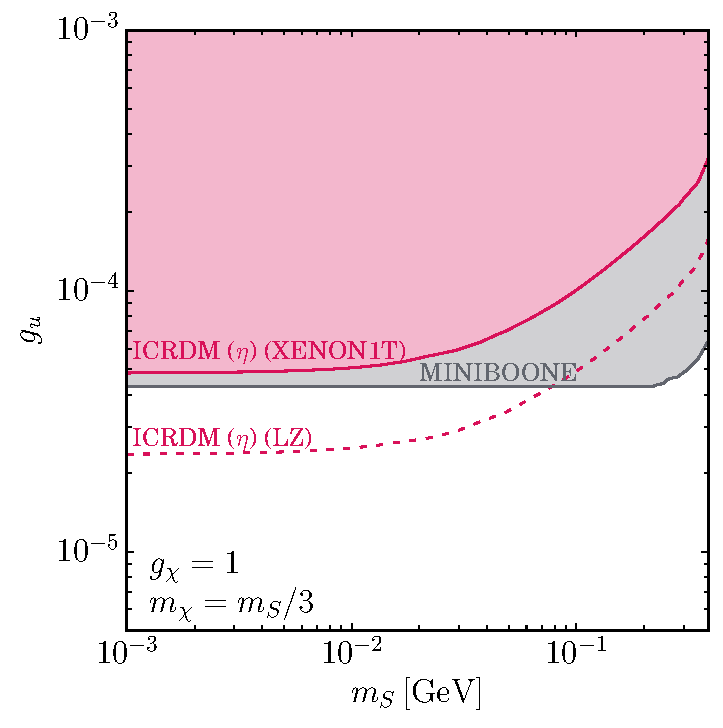
\includegraphics[width=0.6 \textwidth]{hadrophilic_no_title.pdf}
\end{center}
\caption{90\% CL limits from inelastic cosmic ray dark matter flux from $\eta$ decays in red, for a hadrophilic scalar mediator of mass $m_S$ with up-quark coupling $g_u$, setting $g_\chi=1, m_\chi = m_S/3$. The solid line denotes current limits from XENON1T~\cite{Aprile:2018dbl}; the dashed line are future projections for the LZ experiment~\cite{Akerib:2018lyp}. Current MiniBooNE limits from Ref.~\cite{Aguilar-Arevalo:2018wea} are shown in grey.
\label{fig:hadrophilic}}
\end{figure}

Next, we consider the hadrophilic scalar mediator model of Ref.~\cite{Batell:2018fqo}. The singlet scalar $S$ couples to a Dirac fermion dark matter $\chi$ and to the up quark through the Lagrangian terms
%
\begin{align}
\mathcal{L} \supset -g_\chi S\bar{\chi}_L \chi_R - g_u S \bar{u}_L u_R + \text{h.c.} \, .
\end{align}
%
The couplings to other flavours are assumed to be sub-dominant, so that we are left with four free parameters characterising the simplified model: $m_S$, $m_\chi$, $g_u$, and $g_\chi$. The branching ratio of $\eta$ mesons decaying into dark matter is given by 
%
\begin{equation}
BR(\eta \to \pi^0 S) = \frac{C^2 g_u^2 B^2}{16\pi m_\eta \Gamma_\eta} \lambda^{1/2}\left(1, \frac{m_S^2}{m_\eta^2}, \frac{m_\pi^2}{m_\eta^2}\right) \, ,
\end{equation}
%
where $B \simeq m_\pi^2/(m_u+m_d)$, $C \equiv \sqrt{1/3} \cos\theta^\prime -\sqrt{2/3} \sin\theta^\prime$ with $\theta^\prime \simeq -20^\circ$ and $\lambda(a,b,c) = a^2 + b^2 + c^2 -2ab - 2bc - 2ac$. We assume here that $BR(S \to \chi \chi) = 1$. For the differential $\chi$-nucleus cross-section involving a scalar mediator we have 
%
\begin{align}
\frac{d\sigma_{\chi N}}{dT_N} &= \frac{\left(Z y_{Spp} + (A-Z) y_{Snn}\right)^2 g_\chi^2}{8\pi} \nonumber \\
& \times \frac{(2m_N + T_N) (2 m_\chi^2 + m_N T_N)}{(T_\chi^2 + 2m_\chi T_\chi)(2m_N T_N + m_S^2)^2} F_H^2(\sqrt{2 m_N T_N}) \, ,
\end{align}
%
where $Z$ ($A-Z$) are the number of protons (neutrons), $y_{Spp} = 0.014 \cdot g_u m_p/m_u$, $y_{Snn} = 0.012 \cdot g_u m_n/m_u$, and $F_H$ is the Helm form factor~\cite{Duda:2006uk}. Computing the rate as described above, we obtain the 90\% CL limits shown in Fig. \ref{fig:hadrophilic} in red on the $g_u$ vs $m_S$ plane, for $g_\chi = 1, m_\chi = m_S/3$. The Earth suppresses the flux significantly only for values of $g_u$ greater than displayed. The MiniBooNE limits from Ref.~\cite{Batell:2018fqo} are shown in grey. Note that for $g_\chi=1$ the constraints from the E787/E949 experiment are stronger than the MiniBooNE and XENON1T limits~\cite{Batell:2018fqo}; however, they are set by invisible Kaon decays and are independent of $g_\chi$, whereas direct detection constraints from $\eta$ decay sources will grow quadratically with the dark matter coupling.

\section{Summary and Conclusions}

As the search for dark matter broadens, it is becoming increasingly important to maximise every resource that we have, both technological and astrophysical. In this respect cosmic rays provide a valuable tool. It has long been appreciated that cosmic rays are a natural accelerator for probing high energies, or as a background to indirect signals of dark matter decay; here we studied the potential of cosmic rays as a {\it source} of dark matter for direct detection. This opens up the potential of extending the sensitivity of various experiments to explore complementary parameter space, as we have illustrated for the case of XENON1T. It is remarkable that in this example the resulting limits are comparable to dedicated beam dump experiments such as MiniBooNE. These limits will improve in the future with the LZ experiment, by about two orders of magnitude. In forthcoming work we also plan to study the sensitivity of neutrino detectors, as well as cosmic ray production of long-lived hidden sectors that can decay back to Standard Model particles.